\chapter{State-of-the-Art}\label{state-of-the-art}

\section{Cloud Computing}\label{state-of-the-art:s:cloud-computing}

Cloud Computing is a robust and scalable dynamic platform where configurable compute resources are made available as a service, over regular Internet access~\Parencite{alnumay_2020}.
It can also be understood, as the U.S. \gls{nist} indicates as:
\textit{(...) a model for enabling ubiquitous, convenient, on-demand network access to a shared pool of configurable computing resources (e.g., networks, servers, storage, applications, and services) that can be rapidly provisioned and released with minimal management effort or service provider interaction}~\Parencite{mell_grance_2011}. 

According to the predictions in~\Parencite{idc_2021}, \textit{`by the end of 2021, 80\% of enterprises will put a mechanism in place to shift to cloud-centric infrastructure and applications twice as fast as before the [Sars-Cov2] pandemic.'}

Incorrectly used as a synonym of on-demand computing, grid computing or even \gls{saas}~\Parencite{kim_2009}, Cloud Computing has become prevalent nowadays in academic, household and business environments, from small business to large enterprises~\Parencite{rezaei_chiew_lee_shams_aliee_2014} with multiple deployment models:

\subsection{Deployment models for cloud computing}\label{state-of-the-art:ss:deployment-models-for-cloud-computing}

\subsubsection{Private Cloud}\label{state-of-the-art:sss:private-cloud}
A Private Cloud is managed by a single entity, within a single organization. The uses for Private Cloud can be for data privacy reasons, academic reasons, testing reasons or even to utilize existing in-house resources of an organization. This deployment model has the advantage of also allowing local data transfers, which are usually paid for when using other deployment models.

\subsubsection{Community Cloud}\label{state-of-the-art:sss:community-cloud}
A Community Cloud is a Private Cloud where several organizations democratically manage, construct, maintain and share the same cloud infrastructure. This allows for a more economically stable experience.

\subsubsection{Public Cloud}\label{state-of-the-art:sss:public-cloud}
In the Public Cloud, the dominant form of Cloud Computing~\Parencite{dillon_tharam_and_wu_chen_and_chang_elizabeth}, the users are the general public and the owner and maintainer of the underlying infrastructure and services is the cloud service provider. With this cloud, users are provided access to cloud computing services and don't have to worry about the infrastructure.

\subsubsection{Virtual Private Cloud}\label{state-of-the-art:sss:virtual-private-cloud}
A newer type of cloud deployment model has emerged in the last decade where users can experience a mixture of Public and Private Cloud. A \gls{vpc} enables users to manage virtual infrastructure on top of public infrastructure. Cloud providers such as Amazon, Google and Microsoft are the main providers of these \gls{vpc}s~\Parencite{aljamal_el-mousa_jubair_2018}, where users can stipulate the amount and configuration of resources like they were in a Private Cloud, ensuring low to non-existent data transfer limits and cost, more privacy and personalized cloud experiences, while relying on the service provider's public cloud infrastructure.

\subsubsection{Hybrid Cloud}\label{state-of-the-art:sss:hybrid-cloud} 
This deployment model is a combination of one or more of the previous deployment models, where data transfer or task handling can occur seamlessly between the different clouds.

\section{Software-as-a-Service}\label{state-of-the-art:s:software-as-a-service}

Nowadays, with the proliferation of faster Internet connections and the ever-growing landscape of Cloud Computing
\Parencite{dillon_tharam_and_wu_chen_and_chang_elizabeth}, software has become more accessible to companies than before.
By hosting and serving software through the use of Cloud Computing, that software's clients reduce both \gls{capex} and \gls{opex} by eliminating the need to buy and maintain the software and underlying infrastructure~\Parencite{alnumay_2020}.

\gls{saas} allows users to access software and its data, usually hosted on cloud computing services, through thin clients and/or web browsers~\Parencites{mell_grance_2011}{Ali_Abdulrazzaq_and_Md_Sultan_Abu_Bakar_and_abdul_ghani_Abdul_azim_and_Zulzalil_Hazura}. The \textit{Multi-tenancy} design structure of \gls{saas} enables the software to serve multiple users (tenants), from a central server. This design allows for more efficient use of both computer resources and the human resources needed to maintain and manage them, which lowers expenditures and is therefore an imperative for businesses. Through the use of \gls{saas} instead of traditional software, the Clients no longer require the arduous task of deploying software to each one of the users, no longer dealing with varied user endpoint hardware configurations.
Cloud Computing enables ubiquitous access to \gls{saas}, which in turn makes its adoption by businesses more enticing to them. The use of \gls{saas} allows not only for lower \gls{capex} and \gls{opex} for the Client, but also enables faster and more frequent updates of the \gls{saas} (since the software manufacturer has control over it), which increases safety and security for the Client's day-to-day operations~\Parencite{cavusoglu_cavusoglu_zhang_2008}. 

\subsection{Security}\label{state-of-the-art:ss:security}

There have been multiple occasions where security breaches could be prevented had the victims been using up-to-date software~\Parencite{glenn_2018}. The amount of time and resources needed for patching security vulnerabilities varies from company to company but overall, can reach averages of 38 days~\Parencite{rapid7_2018}. By relying on the \gls{saas} provider to patch vulnerabilities in a timely manner, Clients no longer need to allocate costly human resources to this task, which lowers expenses and human error~\Parencite{glenn_2018}. 

The use of a \gls{saas} solution enables the users to access the software and its data without the use of complex networking such as \gls{vpn} and locked-down user endpoints, which have shown its faults when not properly managed, during the SARS-CoV-2 pandemic~\Parencite{adams_al_shahery_chmiel_cunliffe_day_fay_gardner_giuliani_goddard_karl_2022}. By moving the majority of the responsibility for the system's security to the \gls{saas} provider who are more likely to employ security best-practices, it eliminates security threats posed by the Client's deficient security measures.




\section{Software Engineering}\label{state-of-the-art:s:software-engineering}

Software Engineering is the application of engineering to software. It's the \textit{`application of a systematic, disciplined, quantifiable approach to the development, operation and maintenance of software'}. Developing software is a process by which \textit{`user needs are translated into a software product'}~\Parencite{8016712}.

According to the IEEE, this software development process involves the following steps:

\begin{itemize}

    \item Translating user needs into software requirements
    \item Transforming the software requirements into design
    \item Implementing the design in code
    \item Testing the code
    \item Optionally, installing and checking out software for operational use   
\end{itemize}

By following these steps, proper software development can be done in a timely and cost-effective manner.

\subsection{Defining Requirements}\label{state-of-the-art:ss:defining-requirements}

Deciding on what and how to develop software is a difficult part of the software development cycle~\Parencite{pacheco_garcía_reyes_2018}.
By properly defining what the software product requirements are, many software problems can be avoided after the development of the software finishes. Of all defects that software products can have, forty to fifty percent of those defects arise from errors during the first phases of software development: Translating user needs into software requirements and then transforming those into software design~\Parencite{eugene_wiegers_beatty_2013}. 

Requirements specify implementation objectives. They are specifications of the system's behavior, attributes or properties or constraints during the development process~\Parencite{sommerville_sawyer_1997}. Requirements elicitation should be performed during the early stages of the software planning phase in order to prevent major refactoring of code before it's released, which would lead to significant costs for the software development company.

\subsubsection{Identifying Key Stakeholders}\label{state-of-the-art:sss:identifying-key-stakeholders}

Before requirements elicitation, one of the most important steps is asking from whom should such requirements be elicited from. This step is crucial to prevent functional (and financial) success of the project about to be started~\Parencite{lewellen_2020}.


\section{Software Architecture}\label{state-of-the-art:s:software-architecture}

Designing the overall system structure, how the software systems integrate with the infrastructure, how these systems interact with each other and with the users is a considerable challenge for large, complex software systems. Defining the software system, in terms of components and connections between these, is describing the system's software architecture~\Parencite{hasselbring2018software}. Starting from the elicited requirements, and before putting into action the development of the software's code, the next step in software engineering is \textit{Transforming the software requirements into design}. This step allows for easier iteration, since it's a design phase of the software development process, and thus can be modified in a easier and quicker way than performing those changes in an already implemented design.
By producing documentation regarding the software architecture, someone unfamiliar with the whole project can be quickly introduced to the overall structure of the project, without needing to delve deep into the codebase.

\subsection{Service-Oriented Architecture}\label{state-of-the-art:ss:service-oriented-architecture}

There are multiple definitions of \as{soa}~\Parencite{niknejad_ismail_ghani_nazari_bahari_hussin_2020}, but for the context of this piece of work, the definition given in \Parencite{marks2008service} is the most adequate:
\textit{`\as{soa} is a conceptual business architecture where business functionality, or application logic, is
made available to \as{soa} users, or consumers, as shared, reusable services on an IT network. Services
in an \as{soa} are modules of business or application functionality with exposed interfaces, and are
invoked by messages'}

\subsection{Modularity}\label{state-of-the-art:ss:modularity}

Since the early years of software development, there existed the concept of dividing software into modules to improve its comprehensibility and flexibility, while carefully decomposing software in order not to generate too many inefficiencies with this approach~\Parencite{parnas_1972}. Not only are \textit{comprehensibility} and \textit{flexibility} good qualities for the software to possess, but also \textit{dependability}, \textit{maintainability}. These qualities derive from proper software architecture design and implementation and must be contemplated in this phase of software development, as they are too integral to the core software design to be thought of during the software implementation phase. By dividing the software into multiple components and as long as they are not tightly coupled, different developer teams can independently create those components, leading to increased flexibility in software development as well.


\subsection{Reusing Software Components}\label{state-of-the-art:ss:reusing-software-components}

By using modular software architectures, the modular software components are no longer required to be built by the same development team nor being built specifically for a single project. 
Code reuse is a common practice nowadays and, similarly, reusing whole software components in a software architecture introduces the same advantages, by reducing work to be done in order to create a new architecture and implement it and easier and more cost-effective maintenance~\Parencite{hasselbring2018software}. Additionally, it increases system stability, security and reliability when reusing components that have been publicly published and evaluated by the software development community. However, when dealing with 3rd-party components, additional care must be taken to ensure that the evaluation of that software is done on a constant basis and that any changes to that component only reflect on the system after thorough review of said changes. Otherwise, external actors may introduce malicious code in the component before publication and compromise the security of those who rely on that component~\Parencite{tal_2022}.

\subsection{Cohesion and Coupling}\label{state-of-the-art:ss:cohesion-and-coupling}
In software development there two relevant goals during development: \textit{cohesion} and \textit{coupling}, where the first is related to how code is grouped together in a logical unit, the latter is related to how that code is dependent on each other. Ideally, developers nowadays try to develop in order to obtain high cohesion and low coupling~\Parencite{candela_bavota_russo_oliveto_2016}. With high cohesion, developers need not perform code changes in multiple different places to implement new features or fix a bug. With low coupling, those changes are less likely to impact related code.

\subsubsection{Types of Coupling}\label{state-of-the-art:ss:types-of-coupling}


Coupling can happen in multiple, different, manners. Given two components, A and B, if changing the implementation of \textit{A} requires re-implementation of \textit{B}, then there is \textit{implementation coupling}. This is a regular occurence when two components share the same database: if one components changes its database-schema structure, then those changes need to be implemented simultaneously in all other components that rely on the same database-schema structure. This is usually easy to fix, by requiring all components to access the database through a single service, like an \as{api}. If the database-schema needs change, then only the service that serves the database information needs to be changed.


\subsection{Monolithic or Modular and their differences}\label{state-of-the-art:ss:monolithic-or-modular-and-their-differences}

There are multiple, design patterns for software architecture. The most common software architecture, that is generally the first architecture used when developing a new product in a prototype or academic environment is a monolithic architecture. In this kind of architecture, all (or a majority) of the functions of the software are encapsulated in a single software application~\Parencite{chen_li_li_2017}. This monolithic approach makes it easy to develop, test and deploy software, until the amount of functions it encompasses stops being small. When that happens, when the number of functions grows, evolving and updating the software becomes unwieldy. This is due to the high coupling that accompanies monolithic software architectures. In monolithic software architectures, the application's modules cannot be executed independently, changes to a function require the restart of the entire application, usually requiring considerable \textit{downtime}.\footnote{\label{foot:downtime}Time during which the Client doesn't have access to the application}

\begin{figure}[!htbp]
    \centering
    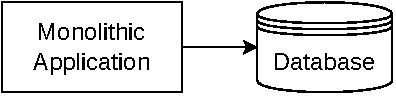
\includegraphics[width=0.40\textwidth]{img/diagrams/pdf/single-process-monolith.drawio.pdf}
    \caption[Single-Process Monolith]{A single-process monolith: all code is packaged into a single process~\Parencite{newman2019monolith}.}
    \label{fig:single-process-monolith}
\end{figure}


When a monolithic application is composed of multiple modules, where these can be developed independently, but still need to be combined for deployment, it's called a modular monolith. 

\begin{figure}[!htbp]
    \centering
    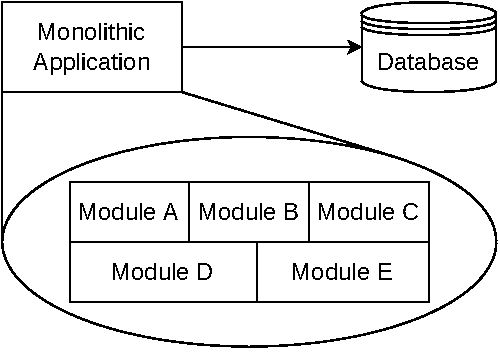
\includegraphics[width=0.50\textwidth]{img/diagrams/pdf/modular-monolith.drawio.pdf}
    \caption[Modular Monolith]{Modular Monolith: application code broken down into modules \parencite{newman2019monolith}.}
    \label{fig:modular-monolith}
\end{figure}







\subsection{Microservices}\label{state-of-the-art:ss:microservices}

Splitting the software system into multiple, independently maintained, fine-grained components, allows developers to deliver software faster and embracing new technologies even faster. By resorting to microservices, new technologies can be tested and prototypes developed in a blink of an eye.
According to~\Parencite{newman_2015}, \textit{`microservices are small, autonomous services that work together'}. While simplistic, this definition sums up quite well what microservices are. Transporting the \gls{srp} in~\Parencite{martin_2014} from classes to microservices, having these fine-grained, independent services allows for more cohesion. As Newman interprets Martin, \textit{`Gather together those things that change for the
same reason, and separate those things that change for different reasons.'}.

\subsubsection{Key Benefits}\label{state-of-the-art:sss:key-benefits}

In a monolithic






According to IDC's predictions~\Parencite{idc_2019}, \textit{`by 2022, 90\% of all new apps will feature microservices architectures that improve the ability to design, debug, update, and leverage third-party code; 35\% of all production apps will be cloud-native'}.















\section{Code Deployment}\label{state-of-the-art:s:code-deployment}




\subsection{DevOps}\label{state-of-the-art:ss:devops}

The \textit{portmanteau} of Development and Operations - DevOps - is as "(...) a set of practices intended to reduce the time between committing a change to a system and the change being placed into normal production, while ensuring high quality", according to~\Parencite{bass_weber_zhu_2015}. There are, therefore, three things to retain from this definition. The two time periods where Development and Deployment occur, the quality of the changes to be committed to a system and the quality of the processes of putting those changes into production~\Parencite{sallin_kropp_anslow_quilty_meier_2021}.

\subsubsection{Development Time}
This time

\section{Observability}\label{state-of-the-art:s:observability}

Virtual Cloud Computing allows users to configure near limitless services, spanning multiple types of resources and with a dynamic range of options for infrastructure. As such, software that relies on \gls{vps}'s elasticity can also become more complex than when using private clouds. With the adoption of modular software design and the increase in the use of micro-services and \textit{serverless} compute services, the complexity of software architecture has increased greatly~\Parencite{niedermaier_koetter_freymann_wagner_2019}.
Such complexity comes at a cost however: Lower Observability. Taking a page from modern control system theory~\Parencite{gopal1993modern}, Observability refers to \textit{the degree to which a system's internal state can be determined from its output}. 
The ability to closely monitor a system's internal state is beneficial during software deployments as well as after them, as it allows stating whether the system is running according to plan.
While a few services can be easily monitored by a single human resource inside a company, complex systems require huge efforts to keep in check on a regular basis. 
Erratic or unexpected system behavior can be spotted when certain patterns make themselves apparent through monitoring. These patterns become difficult to spot when the amount of monitored metrics are inadequate for the system's complexity.
As a means to increase transparency in these new distributed and complex systems, observability tools have emerged that allow for \textit{traces}, \textit{metrics} and \textit{logs} to be generated, collected and further analyzed so that insightful information towards the system's internal state can be attested.

\subsection{OpenTelemetry}\label{state-of-the-art:ss:opentelemetry}

An open-source project, \gls{otel} is a framework born from the software industry's interest on open-source tools, \gls{sdk} and \gls{api} for sending this monitoring data to a Observability back-end in a standardized, vendor-agnostic way~\Parencite{observability_primer_2022}. Before this open-source solution became available, Observability software required the software developers to use that specific Observability back-end's libraries and agents to emit the required data. From a technical and business point-of-view, this was harmful to a software company, since it greatly reduces the ability to quickly and easily change Observability back-end, locking the company in using the same observability software for long periods of time, regardless of the adequacy of it.
With this solution, open-source and innovative add-ons and custom tools to enhance Observability of a system can be made and implemented in much less time, while allowing changing the tools to interact with each other, generating even more insightful knowledge about the systems internal state.

\subsection{Telemetry}\label{state-of-the-art:ss:telemetry}

Telemetry, in the context of this document, refers to the data a system sends regarding its internal state. For software, this data can be in the form of traces, logs and metrics.
\textbf{\textit{Logs}} are timestamped messages emitted by a service or component of a system, which inform about a specific occurrence, such as a request being made to a service or logging the time it took for a function to perform.
\textbf{\textit{Traces}} are data that informs about the path that a request took while it propagates through a service or component. If it traverses more than one service, it is called a \textbf{\textit{distributed trace}}. Distributed traces keep software developers and maintainers informed about the entire path that a request might make, which is a hard task to perform when dealing with multi-service software architectures, like microservice or serverless software architectures. These kinds of architectures are usually complex and non-deterministic, which make debugging quite an endeavor. Individually, these traces and logs provide information about a specific event or set of sub-events that are related to an event. However, in order to ensure system reliability, a system needs to be monitored not just for a single instant but throughout time. This gives an additional dimension to the data emitted by the system's components. By aggregating numeric data over a set period of time, \textbf{\textit{metrics}} can be obtained that give more insightful knowledge regarding the system's internal state. For cases when the information is not numeric in nature, for example a \textit{log} informing that there has been an error, this information can be transformed to inform of the frequency of the event that created that message. Thus, this quantification of data allows for metrics to be recorded and shown graphically, where patterns can be detected. By quantifying telemetry data and generating metrics, it becomes possible to evaluate the system's behavior before, during and after a software deployment so that it's success can be ascertained~\Parencite{mills1988software}
